\documentclass[12pt]{article}
\usepackage[utf8]{inputenc}
\usepackage{upquote}
\usepackage[margin=1in]{geometry} 
\usepackage{amsfonts,amsmath,amsthm,amssymb}
\usepackage{graphicx}
\usepackage{listings}
\usepackage{float}
\usepackage{siunitx}
\newenvironment{statement}[2][Statement]{\begin{trivlist}
\item[\hskip \labelsep {\bfseries #1}\hskip \labelsep {\bfseries #2.}]}{\end{trivlist}}
\usepackage{xcolor}


\usepackage{booktabs}
\usepackage{subfigure}


% Listings package for code rendering (No external dependencies)
\usepackage{listings}  
\usepackage{xcolor}   % Color support
\usepackage{tcolorbox} % Box for better appearance

% Define custom colors for code highlighting
\definecolor{codegreen}{rgb}{0,0.6,0}
\definecolor{codegray}{rgb}{0.5,0.5,0.5}
\definecolor{codepurple}{rgb}{0.58,0,0.82}
\definecolor{backcolour}{rgb}{0.95,0.95,0.92}


\lstset{frame=tb,
    language=Python,
    backgroundcolor=\color{backcolour},   
    commentstyle=\color{codegreen},
    keywordstyle=\color{magenta},
    numberstyle=\tiny\color{codegray},
    stringstyle=\color{codepurple},
    basicstyle=\ttfamily\footnotesize,
    breakatwhitespace=false,         
    breaklines=true,                 
    keepspaces=true,                 
    numbers=left,       
    numbersep=5pt,                  
    showspaces=false,                
    showstringspaces=false,
    showtabs=false,                  
    tabsize=2,
}



\title{Handin 5}

\begin{document}
\maketitle

\section{Introduction}
In this assignment, our main tasks are as follows: 1 Implemented Newtons and Steepest Descent under linear equality constraints.
2 Show the theoretical proof and provide test cases design to ensure the correctness.
3 Designed 4 constraint scenarios to evaluate the performance of the two algorithms and provides visual results.
\section{Theory}
\subsection{Derive the Analytical solution of $min_{\lambda}||\nabla f(x_k) - A^T \lambda ||^2$}

Suppose that, the objective Function: 
\[
\phi (\lambda) = ||\nabla f(x_k) - A^T \lambda ||^2 = (\nabla f(x_k) - A^T\lambda )^\top(\nabla f(x_k) - A^T\lambda)
\]
It is equal to find a $\lambda$ to make $A^T \lambda$ fits $\nabla f(x_k)$.
 Let the gradient to 0:
 \[
 \nabla_\lambda \phi(\lambda) = -2A(\nabla f(x_k) - A^T\lambda) = 0
 \]
 And so we get: $\lambda^* = (AA^T)^{-1}A\nabla f(x_k)$.\\
This is the analytical solution of the problem, and it can be used to compute a stopping criterion because it means the gradient of the feasible direction satisfies the optimality condition.
\subsection{proof of lemma 7}
It is equal to proof (1) 
\[
T_C(x) \subseteq \left\{p\in \mathbb{R}^n : a_i^T p = 0, i = 1, ..., m\right\}
\]
Suppose that, $p \in T_C(x)$, so there will be a sequence $t_k \downarrow 0$ and $p_k \rightarrow p$ to make $x_k = x + t_kp_k \in C$ for all k.
And because $x_k \in C$ so $a_i^T x_k + b = 0$, and we can replace $x_k$ to get:
\[
a_i^T(x + t_kp_k) + b = (a^T_ix + b) + t_k(a_i^Tp_k) = 0
\]
so $t_k(a_i^Tp_k) = 0$ for every k, so $a_i^Tp_k = 0$ because $t_k > 0$ for every k. \\
So when $\lim_{k \rightarrow \infty} a^T_ip_k = 0$ for i = 1, ..., m.so we get (1).\\

(2)
\[
T_C(x) \supseteq \left\{p\in \mathbb{R}^n : a_i^T p = 0, i = 1, ..., m\right\}
\]
suppose that, $a_i^Tp_k = 0, \forall i = 1, .. , m$, we need to proof $p \in T_C(x)$, let $x(t) = x + tp, t\geq 0$.\\
for very $t \geq 0$, check the constraint:
\[
a_i^Tx(t) + b = a^T_i(x + tp) + b = (a^T_i x + b) + t(a_i^Tp) = 0
\]
So $x(t) \in C$, and specially, when $t \rightarrow 0^+$, the derivative of a path:
\[
\frac{d}{dt} x(t) |_{t = 0} = p
\]
so $p \in T_C(x)$, and we can get (2), so we show the lemma 7. 
\section{Experiments}

%Description of the experiments performed.
%Description of procedure and evaluation metrics.
%Also includes choices of parameters
\subsection{experimental setup}
The objective function of our experiment is: 
\[
f(x) = 0.5(x^2_1 + 4x^2_2) - 2x_1 - 8x_2
\]
We designed 4 constraint scenes: 1 $x_1 + x_2 = 0 $ .2 $x_1 - x_2 = 0 $ . 3 $x_1 + x_2 + 1= 0 $. 4 $2x_1 + x_2 = 0 $, To ensure the initial point can fit the constraint, we use SVD to get the minimum norm solution.
\subsection{evaluation procedure}
\textbf{Parameter settings}:\\
Stopping criteria: For the steepest descent method, use $||grad f(x_k) - A^T \lambda^* ||< 1e-6$. For the Newton method, use Newton step size $||p_k|| < 1e-6$.\\
Maximum number of iterations: 100.\\
Backtracking line search parameters: initial step size $\alpha = 1.0$, \\Armijo condition constant $c = 1e-4$, decay factor $\rho = 0.5$\\
\textbf{Experimental steps}\\
For each constraint scenario: \\
1 Calculate the initial point $x_0$ that satisfies the constraint through SVD\\
2 Run the steepest descent method and Newton's method respectively, and record $x_k$, gradient residual, objective function value, step size for each iteration\\
3 Save the data files and graphs such as the iteration trajectory, residual change, objective function value change of each scenario.
\subsection{evaluation metrics}
We use the following indicators to  evaluate the performance objectively: 1 final residual, 2 the number of iterations, 3 Iteration trajectory, 4 convergence curve, 5 Objective function value.
\section{Results and Discussion}
In this section, we will give the results of the 4 scenarios respectively, and discuss the experiment and the experimental shortcomings in the end.
\subsection{$x_1 + x_2 = 0 $}
The initial point of this scenario is (0, 0), and the number of iterations and the final residual of the two algorithms are listed as follow:
\begin{table}[h]
    \centering
    \scalebox{0.8}{ % 
        \begin{tabular}{l p{7cm} p{7cm} } % 
        \toprule
        & steepest descent& newton\\
        \midrule
        iterations& 
        13&
        2\\
        final residual& 2.52e-7& 0\\
        \bottomrule
        \end{tabular}
    }
    \caption{s1}
    \label{tab:s1}
\end{table}

The images of the convergence curve, iteration trajectory and objective function value:\\
\begin{figure}[ht]
\centering
\subfigure[]{
    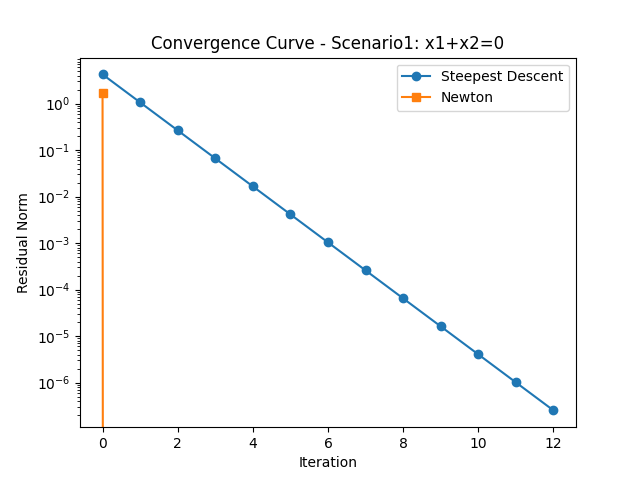
\includegraphics[width=0.3\columnwidth, keepaspectratio]{pics/handin_5/Scenario1_x1+x2=0_convergence.png}
\label{fig:s1}
}
\subfigure[]{
    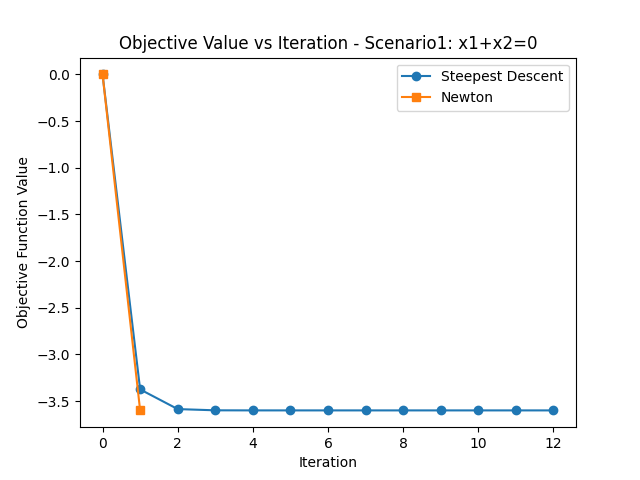
\includegraphics[width=0.3\columnwidth, keepaspectratio]{pics/handin_5/Scenario1_x1+x2=0_objective.png}
    \label{fig:s1}
}
\subfigure[]{
    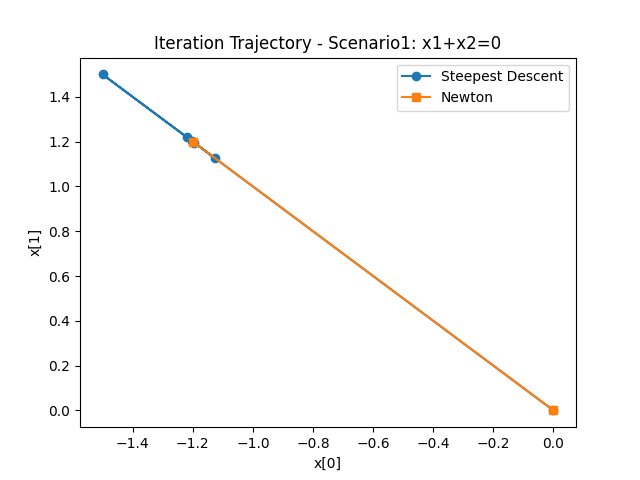
\includegraphics[width=0.3\columnwidth, keepaspectratio]{pics/handin_5/Scenario1_x1+x2=0_trajectory.png}
    \label{fig:s1}
}
\caption[]{convergence curve, iteration point trajectory and objective function value}
\label{fig:s1}
\end{figure}
\subsection{$x_1 - x_2 = 0 $}

The initial point of this scenario is (0, 0), and the number of iterations and the final residual of the two algorithms are listed as follow:\\
\begin{table}[h]
    \centering
    \scalebox{0.8}{ % 
        \begin{tabular}{l p{7cm} p{7cm} } % 
        \toprule
        & steepest descent& newton\\
        \midrule
        iterations& 
        13&
        2\\
        final residual& 4.21e-7& 0\\
        \bottomrule
        \end{tabular}
    }
    \caption{s2}
    \label{tab:s2}
\end{table}

The images of the convergence curve, iteration trajectory and objective function value:\\
\begin{figure}[ht]
\centering
\subfigure[]{
    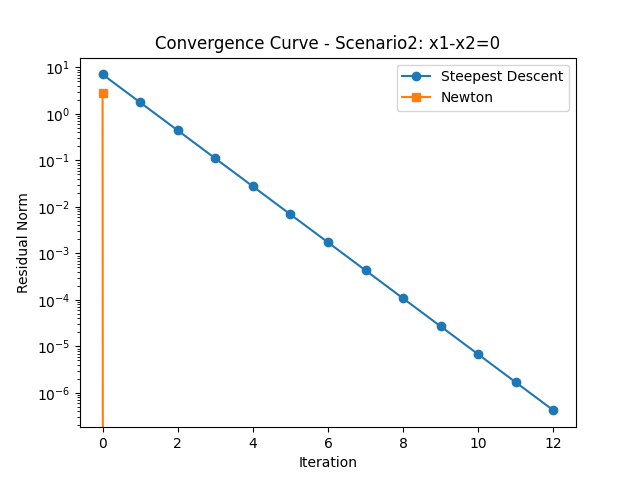
\includegraphics[width=0.3\columnwidth, keepaspectratio]{pics/handin_5/Scenario2_x1-x2=0_convergence.png}
\label{fig:s2}
}
\subfigure[]{
    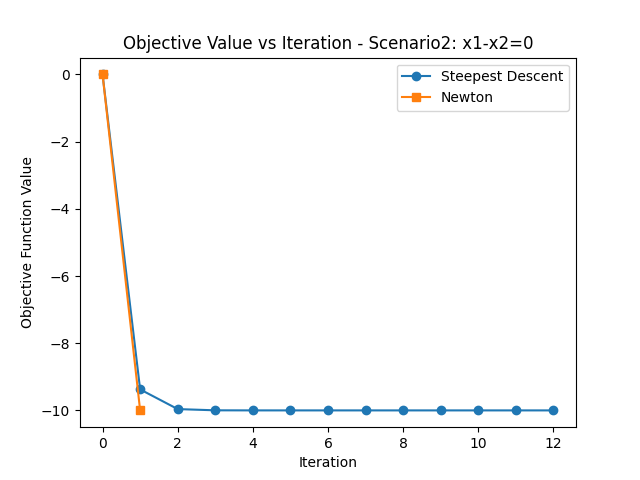
\includegraphics[width=0.3\columnwidth, keepaspectratio]{pics/handin_5/Scenario2_x1-x2=0_objective.png}
    \label{fig:s1}
}
\subfigure[]{
    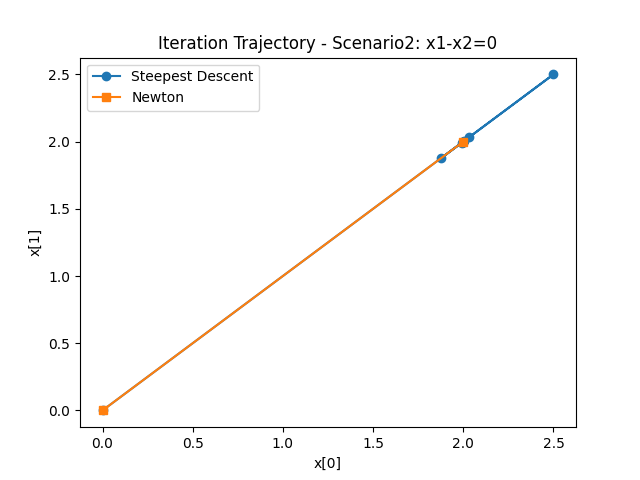
\includegraphics[width=0.3\columnwidth, keepaspectratio]{pics/handin_5/Scenario2_x1-x2=0_trajectory.png}
    \label{fig:s1}
}
\caption[]{convergence curve, iteration point trajectory and objective function value}
\label{fig:s1}
\end{figure}
\subsection{$x_1 + x_2 + 1 = 0 $}

The initial point of this scenario is (-0.49, -0.49), and the number of iterations and the final residual of the two algorithms are listed as follow:\\
\begin{table}[h]
    \centering
    \scalebox{0.8}{ % 
        \begin{tabular}{l p{7cm} p{7cm} } % 
        \toprule
        & steepest descent& newton\\
        \midrule
        iterations& 
        13&
        2\\
        final residual& 3.16e-7& 0\\
        \bottomrule
        \end{tabular}
    }
    \caption{s3}
    \label{tab:s2}
\end{table}

The images of the convergence curve, iteration trajectory and objective function value:\\
\begin{figure}[ht]
\centering
\subfigure[]{
    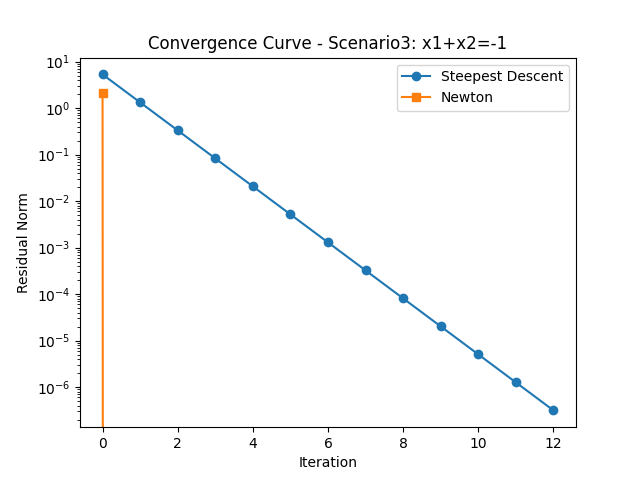
\includegraphics[width=0.3\columnwidth, keepaspectratio]{pics/handin_5/Scenario3_x1+x2=-1_convergence.png}
\label{fig:s2}
}
\subfigure[]{
    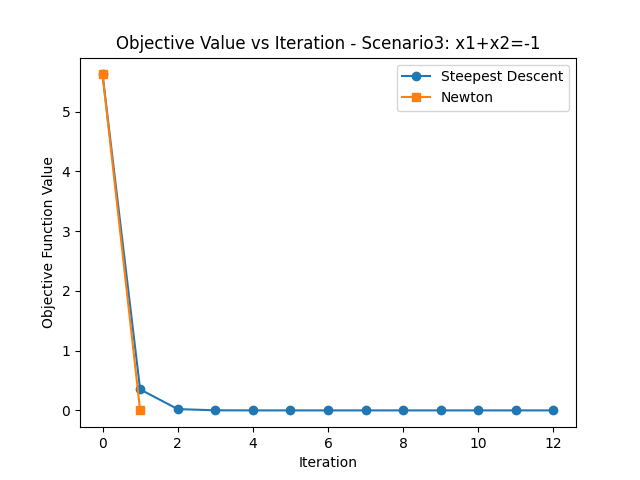
\includegraphics[width=0.3\columnwidth, keepaspectratio]{pics/handin_5/Scenario3_x1+x2=-1_objective.png}
    \label{fig:s1}
}
\subfigure[]{
    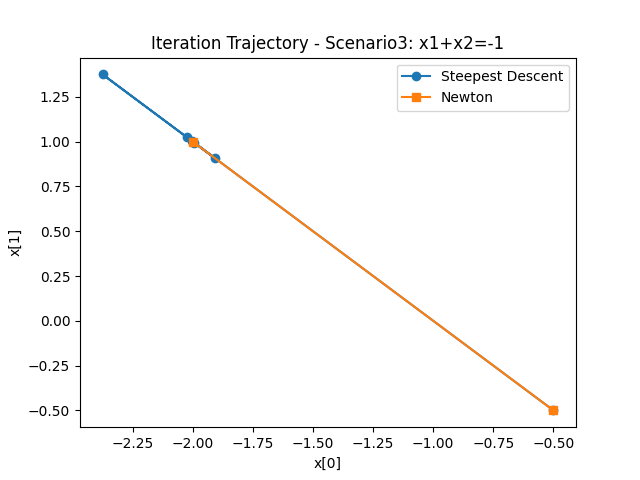
\includegraphics[width=0.3\columnwidth, keepaspectratio]{pics/handin_5/Scenario3_x1+x2=-1_trajectory.png}
    \label{fig:s1}
}
\caption[]{convergence curve, iteration point trajectory and objective function value}
\label{fig:s1}
\end{figure}

\subsection{$2x_1 + x_2 = 0 $}

The initial point of this scenario is (0, 0), and the number of iterations and the final residual of the two algorithms are listed as follow:\\
\begin{table}[h]
    \centering
    \scalebox{0.8}{ % 
        \begin{tabular}{l p{7cm} p{7cm} } % 
        \toprule
        & steepest descent& newton\\
        \midrule
        iterations& 
        45&
        2\\
        final residual& 9.57e-7& e-7\\
        \bottomrule
        \end{tabular}
    }
    \caption{s4}
    \label{tab:s2}
\end{table}

The images of the convergence curve, iteration trajectory and objective function value:\\
\begin{figure}[H]
\centering
\subfigure[]{
    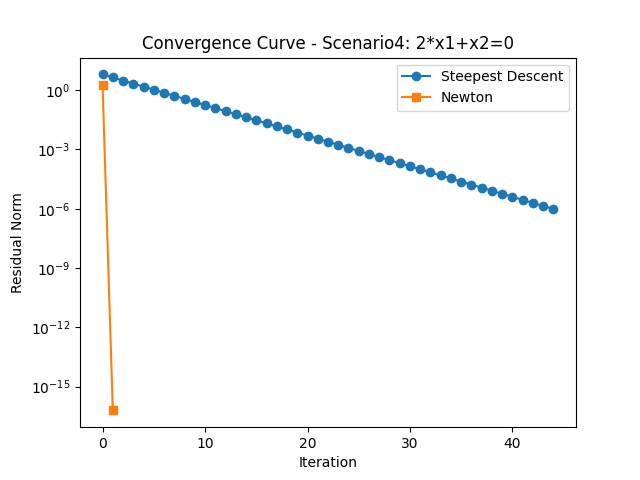
\includegraphics[width=0.3\columnwidth, keepaspectratio]{pics/handin_5/Scenario4_convergence.png}
\label{fig:s2}
}
\subfigure[]{
    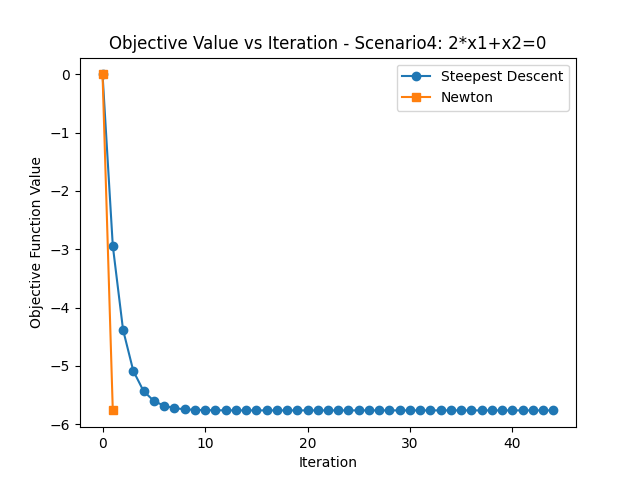
\includegraphics[width=0.3\columnwidth, keepaspectratio]{pics/handin_5/Scenario4_objective.png}
    \label{fig:s1}
}
\subfigure[]{
    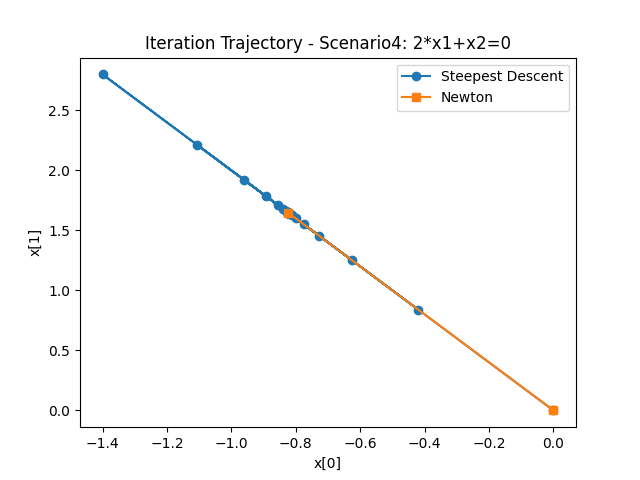
\includegraphics[width=0.3\columnwidth, keepaspectratio]{pics/handin_5/Scenario4_trajectory.png}
    \label{fig:s1}
}
\caption[]{convergence curve, iteration point trajectory and objective function value}
\label{fig:s1}
\end{figure}

\subsection{Discussion}
From the results we can get that in our scenario, newtown performs better than the steepest descent algorithm, and the method's disadvantages are: \textbf{1 Limited problem scale and complexity}: The current experiment only targets two-dimensional quadratic objective functions. it may not be enough to reflect the performance of the algorithm in high-dimensional or more complex problems. \textbf{2 Scenario limitations}: In actual applications, more complex constraints and objective functions may be faced.
\section{Conclusion}
In this assignment, we implemented steepest descent and Newton methods and evaluated their performance using 5 metrics, we derived how to get the stopping criterion. Which deepened our understanding of constrained optimization and numerical algorithm evaluation.


\end{document}
